\chapter{Desarrollo de bloques driver}
\label{cap:capitulo4}
Como ya se ha explicado, VisualCircuit es una plataforma de programación online mediante el uso de bloques, pero para que esté actualizado,
se deben añadir bloques nuevos que ofrezcan esas nuevas funciones y añadirlos a las listas de bloques estándar que la página ofrece.\\
En este capítulo se profundizará en el funcionamiento de la plataforma VisualCircuit así como en el proceso seguido para desarrollar nuevos
bloques para poder añadir ROS2 a la misma.

Los bloques drivers que se van a implementar son para la cámara, el láser y los motores usando un topic de ROS2, ya sea para suscribirse (sensores)
o para publicar (actuadores).\\
A continuación se explica el proceso seguido para desarrollar cada uno de los drivers.

\section{Bloques sensores}
\label{sec:blocks_sensores}

Usando un \textit{input} para activar/desactivar el bloque habilitaremos el uso de máquinas de estados con nuestro bloque.
También queremos compartir la medida del sensor, por lo que añadimos un \textit{output}. Por último, usamos una constante donde definiremos
el \textit{topic} del que obtendremos las lecturas del sensor. Esto lo hacemos para que el usuario no tenga que cambiar el código del bloque para cambiar
el \textit{topic} del que obtiene la información.\\
\begin{figure} [H]
  \begin{center}
      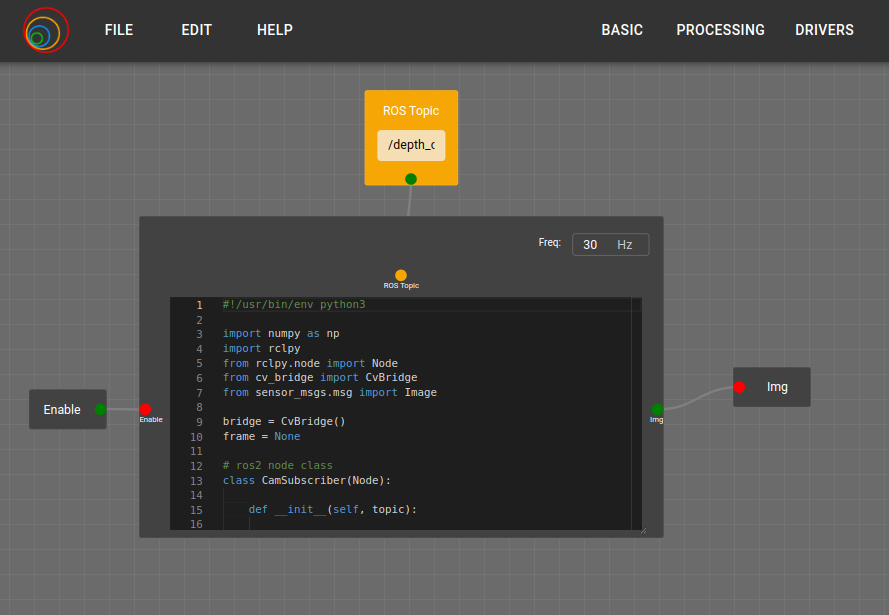
\includegraphics[width=10cm]{figs/c4/VC_driver_blocks.png}
  \end{center}
  \caption[Modelo bloque driver sensores]{Modelo para crear bloques driver de sensores.}
  \label{fig:VC_driver_model}
\end{figure}

En cuanto al código que usaremos, seguiremos las indicaciones de los manuales de
ROS2-humble\footnote{\url{https://docs.ros.org/en/humble/Tutorials/Beginner-Client-Libraries/Writing-A-Simple-Py-Publisher-And-Subscriber.html\#write-the-subscriber-node}}
para usar nodos suscriptores/publicadores con python. El código general para los bloques de sensores (suscriptores) será el siguiente:

\begin{code}[H]
  \begin{lstlisting}[language=python]
    import numpy as np
    import rclpy
    from rclpy.node import Node
    from cv_bridge import CvBridge
    from std_msgs/msg import String #SENSOR MSG TYPE
    
    bridge = CvBridge()
    data = None
    
    # ros2 node class
    class SENSORSubscriber(Node):
        def __init__(self, topic):
            super().__init__('sensor_subscriber')
            self.subscription = self.create_subscription(
              String, topic, self.callback, 10)

            self.subscription  # prevent unused variable warning
    
        def callback(self, msg):
            global data
            # Modify msg as needed and save into global variable
            data = msg

    def main(inputs, outputs, parameters, synchronise):
        global data
        auto_enable = False
        try:
            enable = inputs.read_number('Enable')
        except Exception:
            auto_enable = True
        rclpy.init()
        sensor_sub = SENSORSubscriber(parameters.read_string("ROSTopic"))

        try:
            while auto_enable or inputs.read_number('Enable'):
                data =  None
                rclpy.spin_once(sensor_sub)
                if data is not None:
                    outputs.share_string("Output", data)
                synchronise()
        except Exception as e:
            print('Error:', e)
            pass
        finally:
            print("Exiting")
            synchronise()     
            SENSORSubscriber.destroy_node()
            rclpy.shutdown()
  \end{lstlisting}
  \caption[Modelo de código para bloques drivers]{Modelo de código para bloques drivers.}
  \label{cod:bloques_drivers_sensors_total}
\end{code}

Si lo analizamos por partes, la clase \textbf{\textit{SENSORSubscriber}} (código \ref{cod:bloques_drivers_sensors_node_class}) contiene una función
para inicializar la clase, donde se define el nombre del nodo, se crea el suscriptor y se inicia el suscriptor, y una función callback a la que se
llamará de forma periódica, actualizando el valor de la variable global a la última medida del sensor.

\begin{code}[H]
  \begin{lstlisting}[language=python]
    # ros2 node class
    class SENSORSubscriber(Node):
        def __init__(self, topic):
            super().__init__('sensor_subscriber')
            self.subscription = self.create_subscription(
              String, topic, self.callback, 10)

            self.subscription  # prevent unused variable warning
    
        def callback(self, msg):
            global data
            # Modify msg as needed and save into global variable
            data = msg
  \end{lstlisting}
  \caption[Clase del nodo suscriptor para bloques drivers]{Clase del nodo suscriptor para los bloques drivers.}
  \label{cod:bloques_drivers_sensors_node_class}
\end{code}

En la función main (código \ref{cod:bloques_drivers_sensors_main_general}) tenemos dos partes, la secuencia \textit{try-except} donde se declara
si se está usando una maquina de estados (\textit{enable}) o si debe estar activo constantemente (\textit{autoenable} al haber dado error la lectura
del cable de \textit{enable}).
En la segunda parte (bucle \textit{while}) se reinicia el valor de la variable global y se llama a \textit{``rclpy.spin\_once()"} para obtener la
última medida del sensor y compartirla por el cable \textit{``output"}.

\begin{code}[H]
  \begin{lstlisting}[language=python]
    def main(inputs, outputs, parameters, synchronise):
        global data
        auto_enable = False
        try:
            enable = inputs.read_number('Enable')
        except Exception:
            auto_enable = True
        rclpy.init()
        sensor_sub = SENSORSubscriber(parameters.read_string("ROSTopic"))

        try:
            while auto_enable or inputs.read_number('Enable'):
                data =  None
                rclpy.spin_once(sensor_sub)
                if data is not None:
                    outputs.share_string("Output", data)
  \end{lstlisting}
  \caption[Función main para bloques drivers de sensores]{Función main para los bloques drivers de sensores.}
  \label{cod:bloques_drivers_sensors_main_general}
\end{code}

Una vez que tenemos el modelo general para estos bloques, hay que modificarlos para que funcionen con la cámara y con el láser. Para ello,
cambiaremos el tipo de mensaje que se envía, y haremos que el \textit{callback} obtenga del mensaje de ROS sólo la información que nos interesa,
ya que éste viene con cabeceras y otros datos.\\











































\section{Creación de bloques drivers}
\label{sec:drivers_creacion}

Los bloques drivers que vamos a desarrollar son para implementar la cámara, el láser y los motores usando un topic de ROS2.
Para los sensores (cámara y laser) tenemos que crear la estructura que queremos seguir, ya que ambos serán similares entre sí.\\

Usando un \textit{input} para activar/desactivar el bloque habilitaremos el uso de máquinas de estados con nuestro bloque.
También queremos compartir la medida del sensor, por lo que añadimos un \textit{output}. Por último, usamos una constante donde definiremos
el \textit{topic} del que obtendremos las lecturas del sensor. Esto lo hacemos para que el usuario no tenga que cambiar el código del bloque para cambiar
el \textit{topic} del que obtiene la información.\\
\begin{figure} [H]
  \begin{center}
      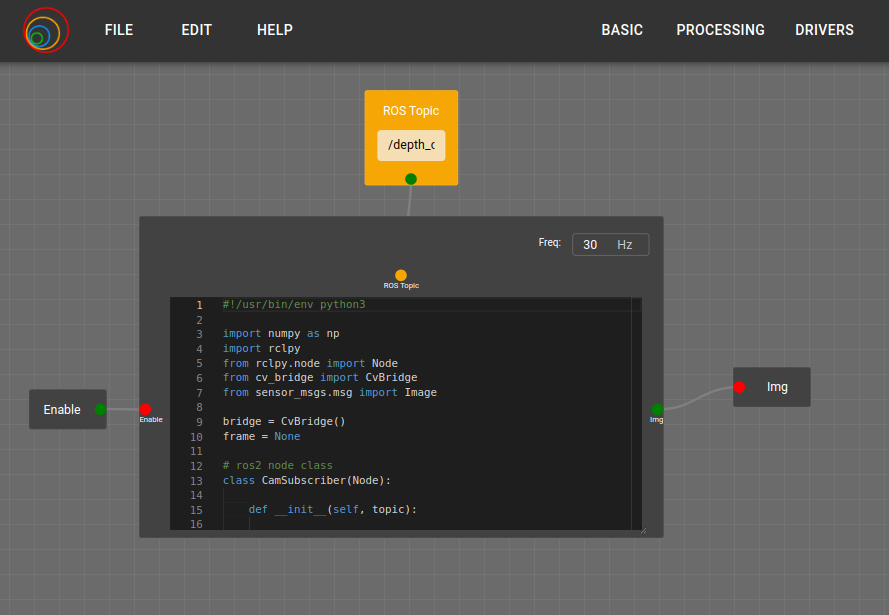
\includegraphics[width=10cm]{figs/c4/VC_driver_blocks.png}
  \end{center}
  \caption[Modelo bloque driver sensores]{Modelo para crear bloques driver de sensores.}
  \label{fig:VC_driver_model}
\end{figure}

En cuanto al código que usaremos, seguiremos las indicaciones de los manuales de
ROS2-humble\footnote{\url{https://docs.ros.org/en/humble/Tutorials/Beginner-Client-Libraries/Writing-A-Simple-Py-Publisher-And-Subscriber.html\#write-the-subscriber-node}}
para usar nodos suscriptores/publicadores con python. El código general para los bloques de sensores (suscriptores) será el siguiente:

\begin{code}[H]
  \begin{lstlisting}[language=python]
    import numpy as np
    import rclpy
    from rclpy.node import Node
    from cv_bridge import CvBridge
    from std_msgs/msg import String #SENSOR MSG TYPE
    
    bridge = CvBridge()
    data = None
    
    # ros2 node class
    class SENSORSubscriber(Node):
        def __init__(self, topic):
            super().__init__('sensor_subscriber')
            self.subscription = self.create_subscription(
              String, topic, self.callback, 10)

            self.subscription  # prevent unused variable warning
    
        def callback(self, msg):
            global data
            # Modify msg as needed and save into global variable
            data = msg

    def main(inputs, outputs, parameters, synchronise):
        global data
        auto_enable = False
        try:
            enable = inputs.read_number('Enable')
        except Exception:
            auto_enable = True
        rclpy.init()
        sensor_sub = SENSORSubscriber(parameters.read_string("ROSTopic"))

        try:
            while auto_enable or inputs.read_number('Enable'):
                data =  None
                rclpy.spin_once(sensor_sub)
                if data is not None:
                    outputs.share_string("Output", data)
                synchronise()
        except Exception as e:
            print('Error:', e)
            pass
        finally:
            print("Exiting")
            synchronise()     
            SENSORSubscriber.destroy_node()
            rclpy.shutdown()
  \end{lstlisting}
  \caption[Modelo de código para bloques drivers]{Modelo de código para bloques drivers.}
  \label{cod:bloques_drivers_sensors_total}
\end{code}

Si lo analizamos por partes, la clase \textbf{\textit{SENSORSubscriber}} (código \ref{cod:bloques_drivers_sensors_node_class}) contiene una función
para inicializar la clase, donde se define el nombre del nodo, se crea el suscriptor y se inicia el suscriptor, y una función callback a la que se
llamará de forma periódica, actualizando el valor de la variable global a la última medida del sensor.

\begin{code}[H]
  \begin{lstlisting}[language=python]
    # ros2 node class
    class SENSORSubscriber(Node):
        def __init__(self, topic):
            super().__init__('sensor_subscriber')
            self.subscription = self.create_subscription(
              String, topic, self.callback, 10)

            self.subscription  # prevent unused variable warning
    
        def callback(self, msg):
            global data
            # Modify msg as needed and save into global variable
            data = msg
  \end{lstlisting}
  \caption[Clase del nodo suscriptor para bloques drivers]{Clase del nodo suscriptor para los bloques drivers.}
  \label{cod:bloques_drivers_sensors_node_class}
\end{code}

En la función main (código \ref{cod:bloques_drivers_sensors_main_general}) tenemos dos partes, la secuencia \textit{try-except} donde se declara
si se está usando una maquina de estados (\textit{enable}) o si debe estar activo constantemente (\textit{autoenable} al haber dado error la lectura
del cable de \textit{enable}).
En la segunda parte (bucle \textit{while}) se reinicia el valor de la variable global y se llama a \textit{``rclpy.spin\_once()"} para obtener la
última medida del sensor y compartirla por el cable \textit{``output"}.

\begin{code}[H]
  \begin{lstlisting}[language=python]
    def main(inputs, outputs, parameters, synchronise):
        global data
        auto_enable = False
        try:
            enable = inputs.read_number('Enable')
        except Exception:
            auto_enable = True
        rclpy.init()
        sensor_sub = SENSORSubscriber(parameters.read_string("ROSTopic"))

        try:
            while auto_enable or inputs.read_number('Enable'):
                data =  None
                rclpy.spin_once(sensor_sub)
                if data is not None:
                    outputs.share_string("Output", data)
  \end{lstlisting}
  \caption[Función main para bloques drivers de sensores]{Función main para los bloques drivers de sensores.}
  \label{cod:bloques_drivers_sensors_main_general}
\end{code}

Una vez que tenemos el modelo general para estos bloques, hay que modificarlos para que funcionen con la cámara y con el láser. Para ello,
cambiaremos el tipo de mensaje que se envía, y haremos que el \textit{callback} obtenga del mensaje de ROS sólo la información que nos interesa,
ya que éste viene con cabeceras y otros datos.\\

% *********CÁMARA
Para el bloque correspondiente a la cámara, el mensaje es del tipo \textit{sensor\_msgs.msg.Image} que, usando el comando``\lstinline|ros2 interface show sensor_msgs/msg/Image|",
podemos ver cuál es su estructura:
\begin{figure} [H]
  \begin{center}
      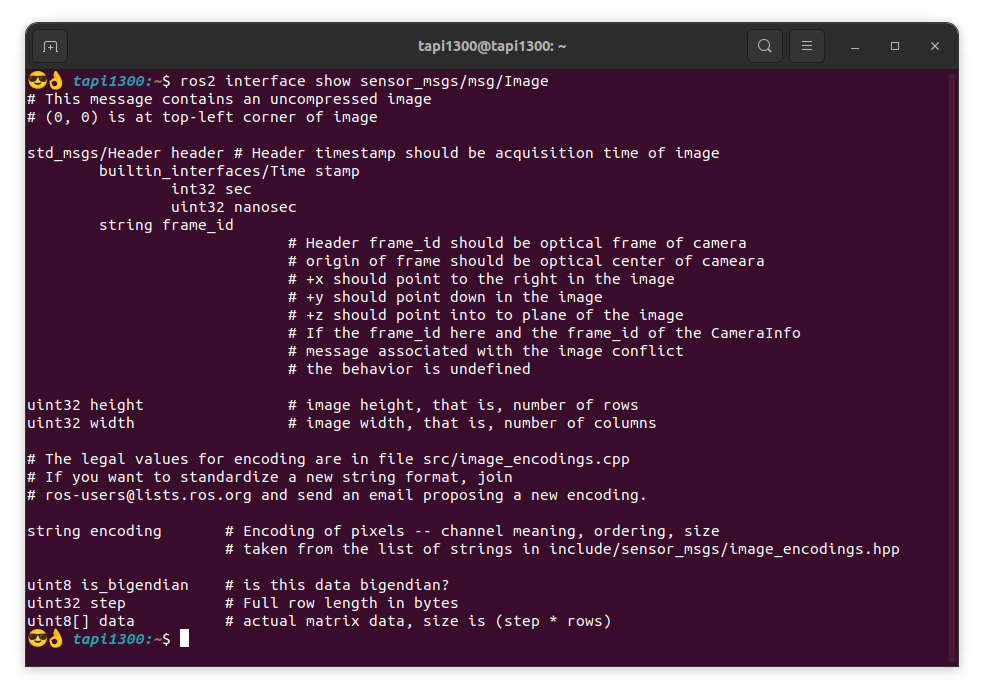
\includegraphics[width=10cm]{figs/c4/image_struct.png}
  \end{center}
  \caption[Estructura mensaje Image]{Estructura del tipo de mensaje \textit{sensor\_msgs/msg/Image}.}
  \label{fig:image_struct}
\end{figure}
Podemos ver en la figura \ref{fig:image_struct} que la imagen que obtendremos estará en el campo \textit{data} del mensaje, pero ROS tiene una
función llamada \textit{CvBridge}\footnote{\textbf{CvBridge}: \url{http://wiki.ros.org/cv_bridge}}, que nos permite transformar un mensaje del
tipo \textit{sensor\_msgs/msg/Image} en una imagen de numpy\footnote{\textbf{Numpy}: \url{https://numpy.org/}}. Como los hilos de VisualCircuit
comparten las imágenes como un array de numpy, debemos convertir la imagen de numpy a un array de numpy, usando la función \textit{numpy.asarray}.
\begin{code}[H]
  \begin{lstlisting}[language=python]
    class CamSubscriber(Node):
        def __init__(self, topic):
            super().__init__('cam_subscriber')
            self.subscription = self.create_subscription(
                Image, topic, self.callback, 10)
            self.subscription  # prevent unused variable warning
        def callback(self, msg):
            global frame
            frame = np.asarray(bridge.imgmsg_to_cv2(msg, "bgr8"), dtype=np.uint8)
  \end{lstlisting}
  \caption[Clase del nodo suscriptor para cámara]{Clase del nodo suscriptor para la cámara.}
  \label{cod:cam_node_class}
\end{code}
En cuanto a la función main, sólo habría que cambiar la función que usamos para compartir, ya que ahora compartimos una imagen:
\begin{code}[H]
  \begin{lstlisting}[language=python]
  while auto_enable or inputs.read_number('Enable'):
      frame =  None
      rclpy.spin_once(camera_subscriber)
      if frame is not None:
          outputs.share_image("Out", frame)
  \end{lstlisting}
  \caption[Cambios main bloque cámara]{Cambios a la función main del bloque driver de la cámara.}
  \label{cod:cam_main_changes}
\end{code}
% ****** LASER
Para el láser, podemos hacer lo mismo que con la cámara y revisar la estructura del tipo de mensaje, en este caso usando ``\lstinline|ros2 interface show sensor_msgs/msg/LaserScan|":
\begin{figure} [H]
  \begin{center}
      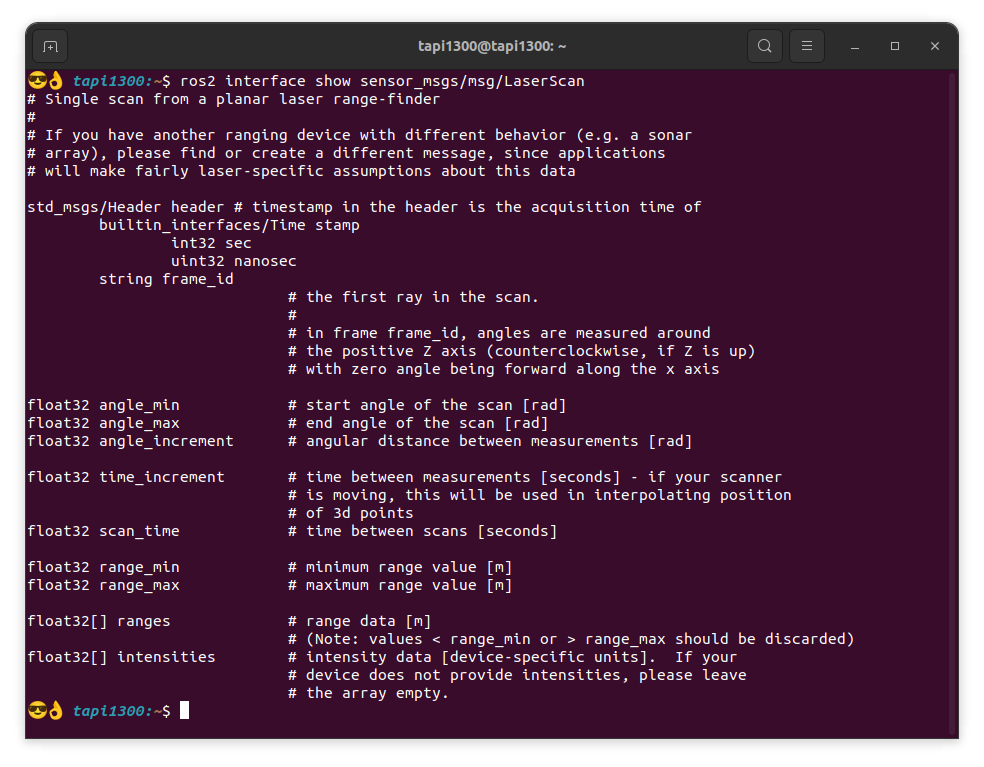
\includegraphics[width=10cm]{figs/c4/laserscan_struct.png}
  \end{center}
  \caption[Estructura mensaje LaserScan]{Estructura del tipo de mensaje \textit{sensor\_msgs/msg/LaserScan}.}
  \label{fig:laserscan_struct}
\end{figure}
Podemos ver en la figura \ref{fig:laserscan_struct} que la lectura del láser estará en el campo \textit{ranges} del mensaje, que es un \textit{array}
de \textit{floats} por lo que, para guardarlo en un array local usaremos la función de python ``\textit{.extend()}", que nos permite añadir una entrada
más a un array. Esto lo haremos en el callback, ya que es donde actualizamos el valor de la variable global.
\begin{code}[H]
  \begin{lstlisting}[language=python]
    class LaserSubscriber(Node):
        def __init__(self, topic):
            super().__init__('laser_subscriber')
            self.subscription = self.create_subscription(
                LaserScan, topic, self.callback, 10)
            self.subscription  # prevent unused variable warning
        def callback(self, msg):
            global measure
            measure = []
            for i in range(len(msg.ranges)):
                measure.extend((str(msg.ranges[i]),))
  \end{lstlisting}
  \caption[Clase del nodo suscriptor para láser]{Clase del nodo suscriptor para el láser.}
  \label{cod:laser_node_class}
\end{code}
En cuanto a la función main, sólo habría que cambiar la función que usamos para compartir, ya que ahora compartimos un array:
\begin{code}[H]
  \begin{lstlisting}[language=python]
    while auto_enable or inputs.read_number('Enable'):
        measure = None
        rclpy.spin_once(laser_subscriber)
        if measure is not None:
            outputs.share_array("Out",measure)   
        synchronise()  
  \end{lstlisting}
  \caption[Cambios main bloque láser]{Cambios a la función main del bloque driver del láser.}
  \label{cod:laser_main_changes}
\end{code}

% ******** MOTOR DRIVER
Ya tenemos los bloques de los sensores, pero aún nos queda el que corresponde a los motores.
En este caso, la configuración del bloque será distinta, ya que no necesitamos salida y sí necesitamos una entrada para que nos
digan qué velocidades mandar al robot. Por esto, tendremos un bloque de código, un parámetro para el \textit{topic} de ROS2 y dos
entradas, una para \textit{enable} (máquinas de estados) y otra para las velocidades que debemos enviar.\\

\newpage
El tipo de mensaje que suelen admitir los robots es ``geometry\_msgs/msg/Twist", y si miramos su estructura usando ``\lstinline|ros2 interface show geometry_msgs/msg/Twist|",
nos encontramos lo siguiente:
\begin{figure} [H]
  \begin{center}
      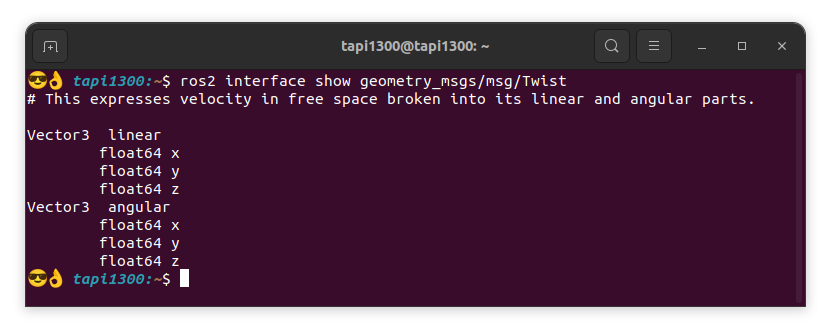
\includegraphics[width=10cm]{figs/c4/twist_struct.png}
  \end{center}
  \caption[Estructura mensaje Twist]{Estructura de tipo de mensaje \textit{geometry\_msgs/msg/Twist}.}
  \label{fig:twist_struct}
\end{figure}

Como podemos ver en la figura \ref{fig:twist_struct}, este tipo de mensajes lleva dos paquetes de 3 floats, el primero para las velocidades
lineales y el segundo para las angulares. Para crear un bloque más general que pueda adaptarse a todo tipo de robots, el bloque recibirá un array
de 6 floats permitiendo introducir velocidades lineales y angulares en las 3 dimensiones que nos permite el mensaje, ya que aunque la mayoría de
robots terrestres sólo usen una velocidad lineal y una angular, así permitimos el uso de este bloque con otros robots como drones o robots con ruedas
omnidireccionales.\\

Para poder crear el nodo publicador iremos, al igual que hicimos con el suscriptor, a los manuales de
ROS2-humble\footnote{\url{https://docs.ros.org/en/humble/Tutorials/Beginner-Client-Libraries/Writing-A-Simple-Py-Publisher-And-Subscriber.html\#write-the-publisher-node}} y
a partir de ahí crear nuestro nodo publicador.













\begin{code}[H]
  \begin{lstlisting}[language=python]
    import numpy as np
    import rclpy
    from rclpy.node import Node
    from cv_bridge import CvBridge
    from geometry_msgs.msg import Twist

    bridge = CvBridge()
    velocities = 0

  \end{lstlisting}
\end{code}
\begin{code}[H]
  \begin{lstlisting}[language=python]
    # ros2 node class
    class VelPublisher(Node):
        def __init__(self, topic):
            super().__init__('vel_publisher')
            self.publisher_ = self.create_publisher(Twist, topic, 1)
            timer_period = 0.5  # seconds
            self.timer = self.create_timer(timer_period, self.timer_callback)
        def timer_callback(self):
            global velocities
            msg = Twist()
            try:
                msg.linear.x = float(velocities[0])
                msg.linear.y = float(velocities[1])
                msg.linear.z = float(velocities[2])
                msg.angular.x = float(velocities[3])
                msg.angular.y = float(velocities[4])
                msg.angular.z = float(velocities[5])
            except IndexError:
                print("bad length for input array")
                return
            self.publisher_.publish(msg)

    def main(inputs, outputs, parameters, synchronise):
        global velocities
        auto_enable = False
        try:
            enable = inputs.read_number('Enable')
        except Exception:
            auto_enable = True
        rclpy.init()
        vel_publisher = VelPublisher(parameters.read_string('ROSTopic'))
        try:
            while auto_enable or inputs.read_number('Enable'):
                velocities = inputs.read_array('Vels')
                if velocities != None:
                    rclpy.spin_once(vel_publisher) 
                synchronise()   
        except KeyboardInterrupt:
            vel_publisher.destroy_node()
            rclpy.shutdown()
  \end{lstlisting}
  \caption[Bloque MotorDriverROS2]{Bloque MotorDriverROS2 completo.}
  \label{cod:motordriverros2_all}
\end{code}

Al ser un publicador, funciona con un temporizador para publicar el mensaje actualizado. Como podemos ver, se lee un array, se guarda en
la variable global y cuando vuelva a ejecutarse el temporizador, se enviará la última actualización de las velocidades.













